\begin{question}
\noindent A UI/UX designer is creating a symmetrical icon for an app. She draws quadrilateral $Q$ on a coordinate grid, then reflects it in the line $y = x$ to create a mirror-image icon $Q'$.

\begin{center}
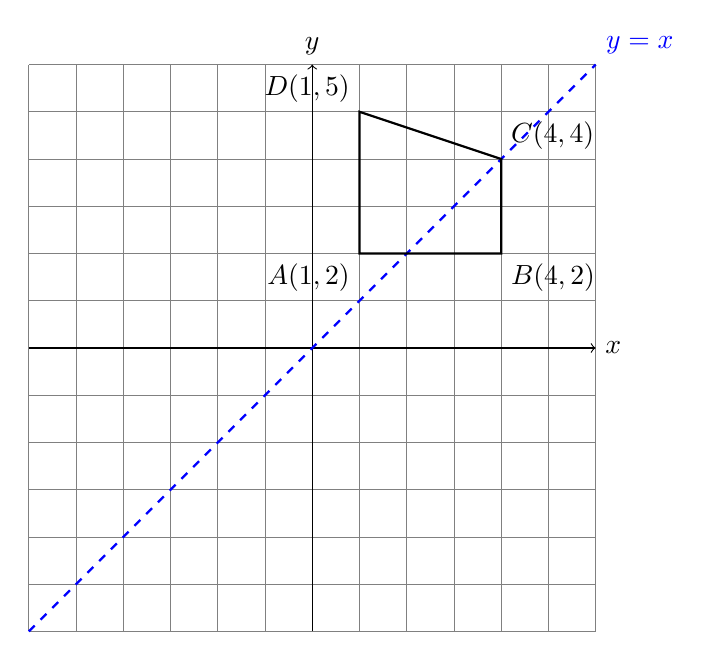
\begin{tikzpicture}[scale=0.6]
    \draw[step=1cm, gray, very thin] (-6,-6) grid (6,6);
    \draw[->] (-6,0) -- (6,0) node[right] {$x$};
    \draw[->] (0,-6) -- (0,6) node[above] {$y$};

    % Line y = x
    \draw[dashed, thick, blue] (-6,-6) -- (6,6) node[above right] {$y=x$};

    % Quadrilateral Q
    \draw[thick] (1,2) -- (4,2) -- (4,4) -- (1,5) -- cycle;
    \node at (1,2) [below left] {$A(1,2)$};
    \node at (4,2) [below right] {$B(4,2)$};
    \node at (4,4) [above right] {$C(4,4)$};
    \node at (1,5) [above left] {$D(1,5)$};
\end{tikzpicture}
\end{center}

\noindent Quadrilateral $Q$ has vertices $A(1,2)$, $B(4,2)$, $C(4,4)$ and $D(1,5)$.

\noindent Reflect quadrilateral $Q$ in the line $y = x$ to give quadrilateral $Q'$.

\noindent Write down the coordinates of the vertices of $Q'$.

\vspace{4cm}

\begin{flushright}
\answerplain{2}
\end{flushright}
\end{question}
